% Grafo agéntico real del sistema PFINAL_AP-IA (LangGraph).
% Refleja la topología compilada en src/agents/orchestrator/graph.py:
%   START -> orchestrator (router LLM)
%   orchestrator -> {analyst, security, registrar, conversational}   [condicional]
%   {analyst, security, registrar} -> orchestrator                   [narrar/encadenar]
%   conversational -> END
%   orchestrator -> END                                              [ask_user / respond_final]
%
% Compilar como figura suelta:
%   pdflatex -interaction=nonstopmode agent_graph.tex
% Incluir desde main.tex:
%   % Grafo agéntico real del sistema PFINAL_AP-IA (LangGraph).
% Refleja la topología compilada en src/agents/orchestrator/graph.py:
%   START -> orchestrator (router LLM)
%   orchestrator -> {analyst, security, registrar, conversational}   [condicional]
%   {analyst, security, registrar} -> orchestrator                   [narrar/encadenar]
%   conversational -> END
%   orchestrator -> END                                              [ask_user / respond_final]
%
% Compilar como figura suelta:
%   pdflatex -interaction=nonstopmode agent_graph.tex
% Incluir desde main.tex:
%   % Grafo agéntico real del sistema PFINAL_AP-IA (LangGraph).
% Refleja la topología compilada en src/agents/orchestrator/graph.py:
%   START -> orchestrator (router LLM)
%   orchestrator -> {analyst, security, registrar, conversational}   [condicional]
%   {analyst, security, registrar} -> orchestrator                   [narrar/encadenar]
%   conversational -> END
%   orchestrator -> END                                              [ask_user / respond_final]
%
% Compilar como figura suelta:
%   pdflatex -interaction=nonstopmode agent_graph.tex
% Incluir desde main.tex:
%   % Grafo agéntico real del sistema PFINAL_AP-IA (LangGraph).
% Refleja la topología compilada en src/agents/orchestrator/graph.py:
%   START -> orchestrator (router LLM)
%   orchestrator -> {analyst, security, registrar, conversational}   [condicional]
%   {analyst, security, registrar} -> orchestrator                   [narrar/encadenar]
%   conversational -> END
%   orchestrator -> END                                              [ask_user / respond_final]
%
% Compilar como figura suelta:
%   pdflatex -interaction=nonstopmode agent_graph.tex
% Incluir desde main.tex:
%   \input{figures/agent_graph.tex}  % dentro de un entorno figure
\documentclass[tikz,border=8pt]{standalone}
\usepackage[T1]{fontenc}
\usepackage{lmodern}
\usetikzlibrary{arrows.meta, positioning, shapes.geometric, calc}

\begin{document}
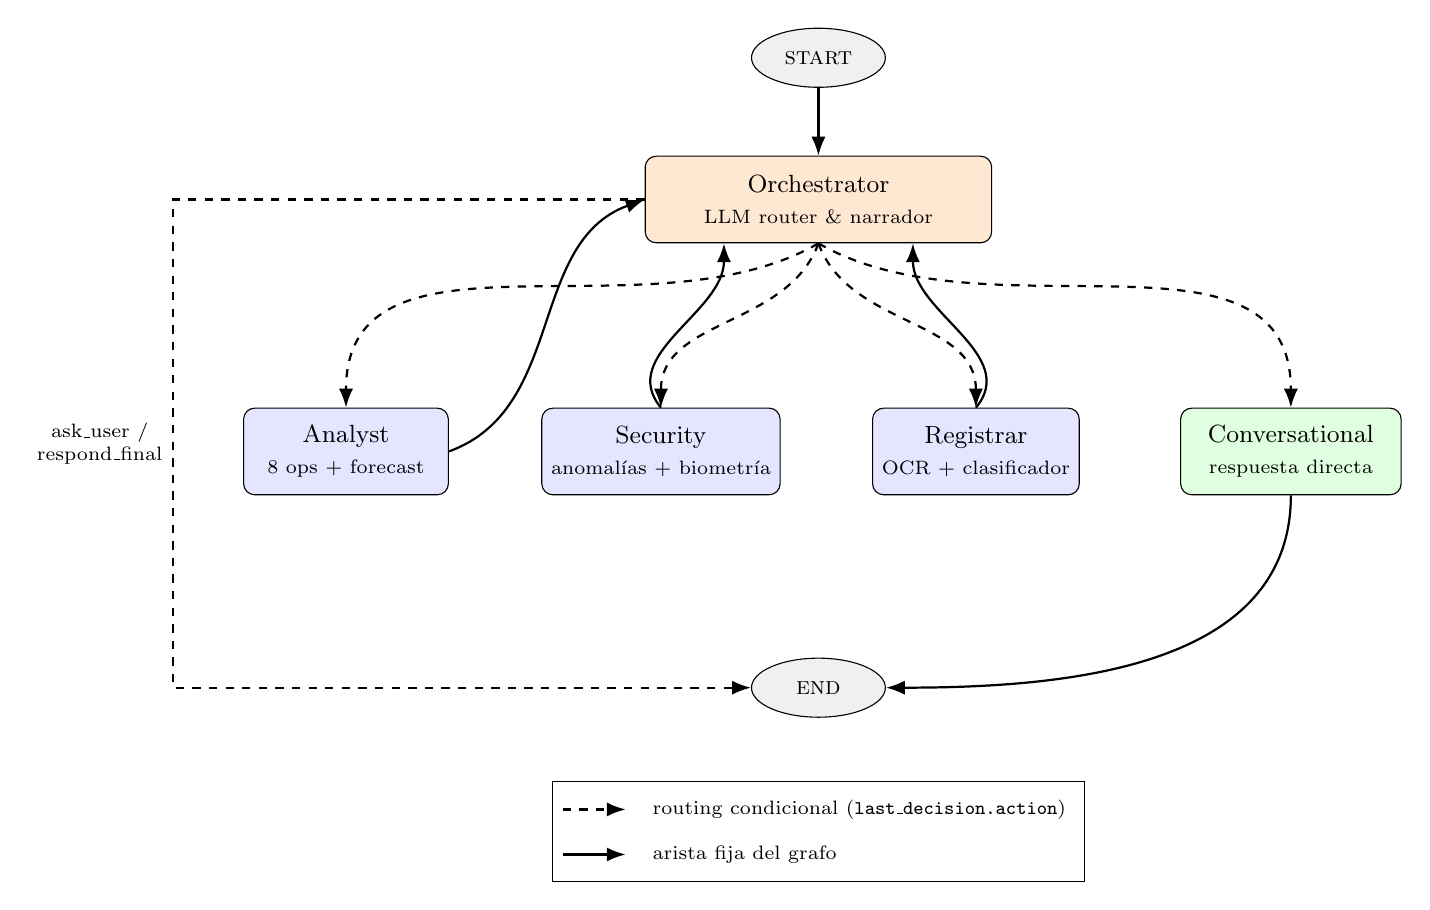
\begin{tikzpicture}[
    >={Latex[length=2.4mm]},
    every node/.style={font=\small},
    terminal/.style={ellipse, draw, fill=gray!12, minimum width=1.7cm, minimum height=0.75cm},
    orch/.style={rectangle, draw, rounded corners, fill=orange!18,
                 minimum width=4.4cm, minimum height=1.1cm, align=center},
    agent/.style={rectangle, draw, rounded corners, fill=blue!10,
                  minimum width=2.6cm, minimum height=1.1cm, align=center},
    convo/.style={rectangle, draw, rounded corners, fill=green!12,
                  minimum width=2.8cm, minimum height=1.1cm, align=center},
    route/.style={->, thick, dashed},
    back/.style={->, thick},
    final/.style={->, thick, dashed}
]

    % --- Fila 0: START ---
    \node[terminal] (start) at (0, 0) {\textsc{start}};

    % --- Fila 1: Orchestrator ---
    \node[orch] (orch) at (0, -1.8)
        {Orchestrator\\\scriptsize{LLM router \& narrador}};

    % --- Fila 2: Agentes (cuatro columnas, centradas en x=0) ---
    \node[agent] (analyst)   at (-6.0, -5.0) {Analyst\\\scriptsize{8 ops + forecast}};
    \node[agent] (security)  at (-2.0, -5.0) {Security\\\scriptsize{anomalías + biometría}};
    \node[agent] (registrar) at ( 2.0, -5.0) {Registrar\\\scriptsize{OCR + clasificador}};
    \node[convo] (conv)      at ( 6.0, -5.0) {Conversational\\\scriptsize{respuesta directa}};

    % --- Fila 3: END ---
    \node[terminal] (end) at (0, -8.0) {\textsc{end}};

    % --- Aristas ---
    % START -> Orchestrator
    \draw[back] (start) -- (orch);

    % Routing condicional (orchestrator -> especialistas)
    \draw[route] (orch.south) to[out=-150, in=90] (analyst.north);
    \draw[route] (orch.south) to[out=-110, in=90] (security.north);
    \draw[route] (orch.south) to[out=-70,  in=90] (registrar.north);
    \draw[route] (orch.south) to[out=-30,  in=90] (conv.north);

    % Retorno de especialistas al orquestador (arista fija)
    \draw[back] (analyst.east)    to[out=20,  in=200] (orch.west);
    \draw[back] (security.north)  to[out=130, in=-90] ($(orch.south)+(-1.2,0)$);
    \draw[back] (registrar.north) to[out=50,  in=-90] ($(orch.south)+(1.2,0)$);

    % Conversational -> END (arista fija)
    \draw[back] (conv.south) to[out=-90, in=0] (end.east);

    % Orchestrator -> END (ask_user / respond_final) — ruta exterior por la
    % izquierda, pasando fuera del nodo Analyst (x = -6.0, ancho 2.6).
    \coordinate (askL) at (-8.2, -1.8);
    \coordinate (askD) at (-8.2, -8.0);
    \draw[final] (orch.west) -- (askL) --
        node[left, font=\scriptsize, align=center]
        {ask\_user /\\respond\_final} (askD) -- (end.west);

    % --- Leyenda ---
    \matrix [draw, below=0.8cm of end, row sep=3pt, column sep=6pt,
             nodes={font=\scriptsize, anchor=west}] {
        \draw[route] (0,0) -- (0.8,0); & \node {routing condicional (\texttt{last\_decision.action})}; \\
        \draw[back]  (0,0) -- (0.8,0); & \node {arista fija del grafo}; \\
    };

\end{tikzpicture}
\end{document}
  % dentro de un entorno figure
\documentclass[tikz,border=8pt]{standalone}
\usepackage[T1]{fontenc}
\usepackage{lmodern}
\usetikzlibrary{arrows.meta, positioning, shapes.geometric, calc}

\begin{document}
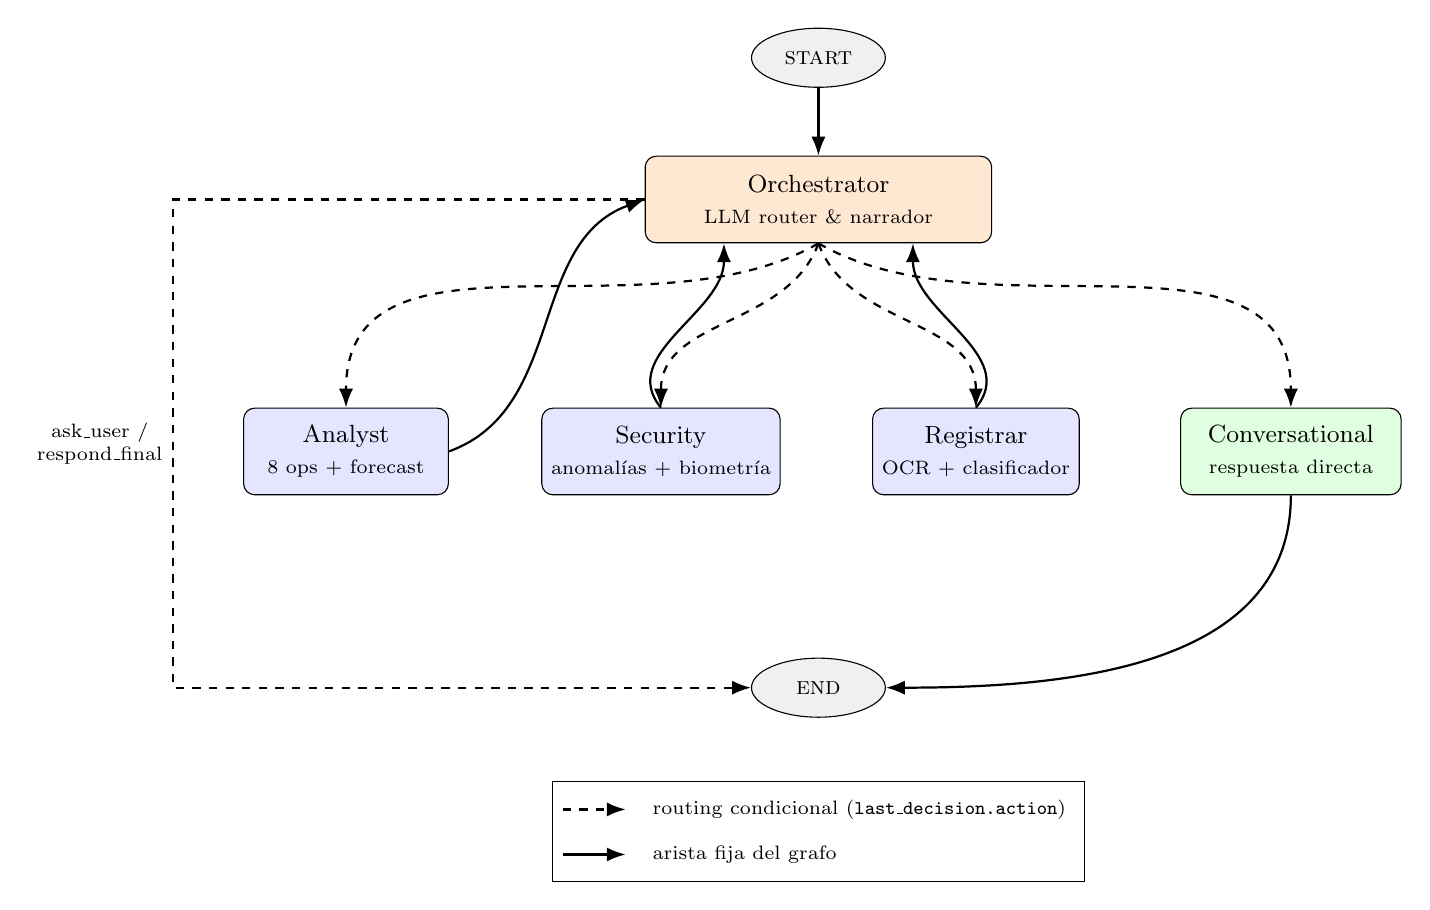
\begin{tikzpicture}[
    >={Latex[length=2.4mm]},
    every node/.style={font=\small},
    terminal/.style={ellipse, draw, fill=gray!12, minimum width=1.7cm, minimum height=0.75cm},
    orch/.style={rectangle, draw, rounded corners, fill=orange!18,
                 minimum width=4.4cm, minimum height=1.1cm, align=center},
    agent/.style={rectangle, draw, rounded corners, fill=blue!10,
                  minimum width=2.6cm, minimum height=1.1cm, align=center},
    convo/.style={rectangle, draw, rounded corners, fill=green!12,
                  minimum width=2.8cm, minimum height=1.1cm, align=center},
    route/.style={->, thick, dashed},
    back/.style={->, thick},
    final/.style={->, thick, dashed}
]

    % --- Fila 0: START ---
    \node[terminal] (start) at (0, 0) {\textsc{start}};

    % --- Fila 1: Orchestrator ---
    \node[orch] (orch) at (0, -1.8)
        {Orchestrator\\\scriptsize{LLM router \& narrador}};

    % --- Fila 2: Agentes (cuatro columnas, centradas en x=0) ---
    \node[agent] (analyst)   at (-6.0, -5.0) {Analyst\\\scriptsize{8 ops + forecast}};
    \node[agent] (security)  at (-2.0, -5.0) {Security\\\scriptsize{anomalías + biometría}};
    \node[agent] (registrar) at ( 2.0, -5.0) {Registrar\\\scriptsize{OCR + clasificador}};
    \node[convo] (conv)      at ( 6.0, -5.0) {Conversational\\\scriptsize{respuesta directa}};

    % --- Fila 3: END ---
    \node[terminal] (end) at (0, -8.0) {\textsc{end}};

    % --- Aristas ---
    % START -> Orchestrator
    \draw[back] (start) -- (orch);

    % Routing condicional (orchestrator -> especialistas)
    \draw[route] (orch.south) to[out=-150, in=90] (analyst.north);
    \draw[route] (orch.south) to[out=-110, in=90] (security.north);
    \draw[route] (orch.south) to[out=-70,  in=90] (registrar.north);
    \draw[route] (orch.south) to[out=-30,  in=90] (conv.north);

    % Retorno de especialistas al orquestador (arista fija)
    \draw[back] (analyst.east)    to[out=20,  in=200] (orch.west);
    \draw[back] (security.north)  to[out=130, in=-90] ($(orch.south)+(-1.2,0)$);
    \draw[back] (registrar.north) to[out=50,  in=-90] ($(orch.south)+(1.2,0)$);

    % Conversational -> END (arista fija)
    \draw[back] (conv.south) to[out=-90, in=0] (end.east);

    % Orchestrator -> END (ask_user / respond_final) — ruta exterior por la
    % izquierda, pasando fuera del nodo Analyst (x = -6.0, ancho 2.6).
    \coordinate (askL) at (-8.2, -1.8);
    \coordinate (askD) at (-8.2, -8.0);
    \draw[final] (orch.west) -- (askL) --
        node[left, font=\scriptsize, align=center]
        {ask\_user /\\respond\_final} (askD) -- (end.west);

    % --- Leyenda ---
    \matrix [draw, below=0.8cm of end, row sep=3pt, column sep=6pt,
             nodes={font=\scriptsize, anchor=west}] {
        \draw[route] (0,0) -- (0.8,0); & \node {routing condicional (\texttt{last\_decision.action})}; \\
        \draw[back]  (0,0) -- (0.8,0); & \node {arista fija del grafo}; \\
    };

\end{tikzpicture}
\end{document}
  % dentro de un entorno figure
\documentclass[tikz,border=8pt]{standalone}
\usepackage[T1]{fontenc}
\usepackage{lmodern}
\usetikzlibrary{arrows.meta, positioning, shapes.geometric, calc}

\begin{document}
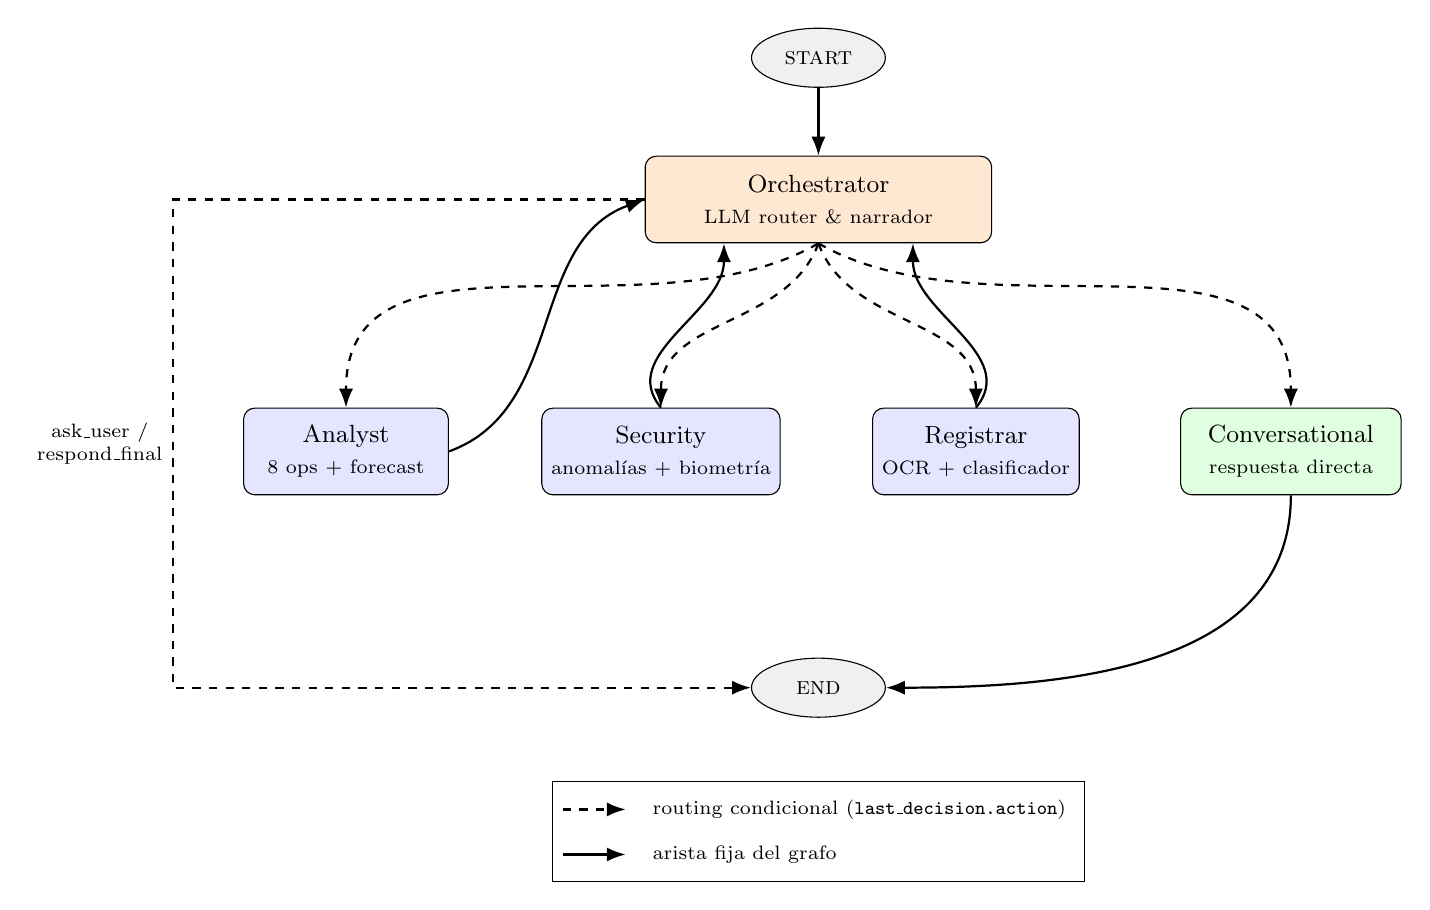
\begin{tikzpicture}[
    >={Latex[length=2.4mm]},
    every node/.style={font=\small},
    terminal/.style={ellipse, draw, fill=gray!12, minimum width=1.7cm, minimum height=0.75cm},
    orch/.style={rectangle, draw, rounded corners, fill=orange!18,
                 minimum width=4.4cm, minimum height=1.1cm, align=center},
    agent/.style={rectangle, draw, rounded corners, fill=blue!10,
                  minimum width=2.6cm, minimum height=1.1cm, align=center},
    convo/.style={rectangle, draw, rounded corners, fill=green!12,
                  minimum width=2.8cm, minimum height=1.1cm, align=center},
    route/.style={->, thick, dashed},
    back/.style={->, thick},
    final/.style={->, thick, dashed}
]

    % --- Fila 0: START ---
    \node[terminal] (start) at (0, 0) {\textsc{start}};

    % --- Fila 1: Orchestrator ---
    \node[orch] (orch) at (0, -1.8)
        {Orchestrator\\\scriptsize{LLM router \& narrador}};

    % --- Fila 2: Agentes (cuatro columnas, centradas en x=0) ---
    \node[agent] (analyst)   at (-6.0, -5.0) {Analyst\\\scriptsize{8 ops + forecast}};
    \node[agent] (security)  at (-2.0, -5.0) {Security\\\scriptsize{anomalías + biometría}};
    \node[agent] (registrar) at ( 2.0, -5.0) {Registrar\\\scriptsize{OCR + clasificador}};
    \node[convo] (conv)      at ( 6.0, -5.0) {Conversational\\\scriptsize{respuesta directa}};

    % --- Fila 3: END ---
    \node[terminal] (end) at (0, -8.0) {\textsc{end}};

    % --- Aristas ---
    % START -> Orchestrator
    \draw[back] (start) -- (orch);

    % Routing condicional (orchestrator -> especialistas)
    \draw[route] (orch.south) to[out=-150, in=90] (analyst.north);
    \draw[route] (orch.south) to[out=-110, in=90] (security.north);
    \draw[route] (orch.south) to[out=-70,  in=90] (registrar.north);
    \draw[route] (orch.south) to[out=-30,  in=90] (conv.north);

    % Retorno de especialistas al orquestador (arista fija)
    \draw[back] (analyst.east)    to[out=20,  in=200] (orch.west);
    \draw[back] (security.north)  to[out=130, in=-90] ($(orch.south)+(-1.2,0)$);
    \draw[back] (registrar.north) to[out=50,  in=-90] ($(orch.south)+(1.2,0)$);

    % Conversational -> END (arista fija)
    \draw[back] (conv.south) to[out=-90, in=0] (end.east);

    % Orchestrator -> END (ask_user / respond_final) — ruta exterior por la
    % izquierda, pasando fuera del nodo Analyst (x = -6.0, ancho 2.6).
    \coordinate (askL) at (-8.2, -1.8);
    \coordinate (askD) at (-8.2, -8.0);
    \draw[final] (orch.west) -- (askL) --
        node[left, font=\scriptsize, align=center]
        {ask\_user /\\respond\_final} (askD) -- (end.west);

    % --- Leyenda ---
    \matrix [draw, below=0.8cm of end, row sep=3pt, column sep=6pt,
             nodes={font=\scriptsize, anchor=west}] {
        \draw[route] (0,0) -- (0.8,0); & \node {routing condicional (\texttt{last\_decision.action})}; \\
        \draw[back]  (0,0) -- (0.8,0); & \node {arista fija del grafo}; \\
    };

\end{tikzpicture}
\end{document}
  % dentro de un entorno figure
\documentclass[tikz,border=8pt]{standalone}
\usepackage[T1]{fontenc}
\usepackage{lmodern}
\usetikzlibrary{arrows.meta, positioning, shapes.geometric, calc}

\begin{document}
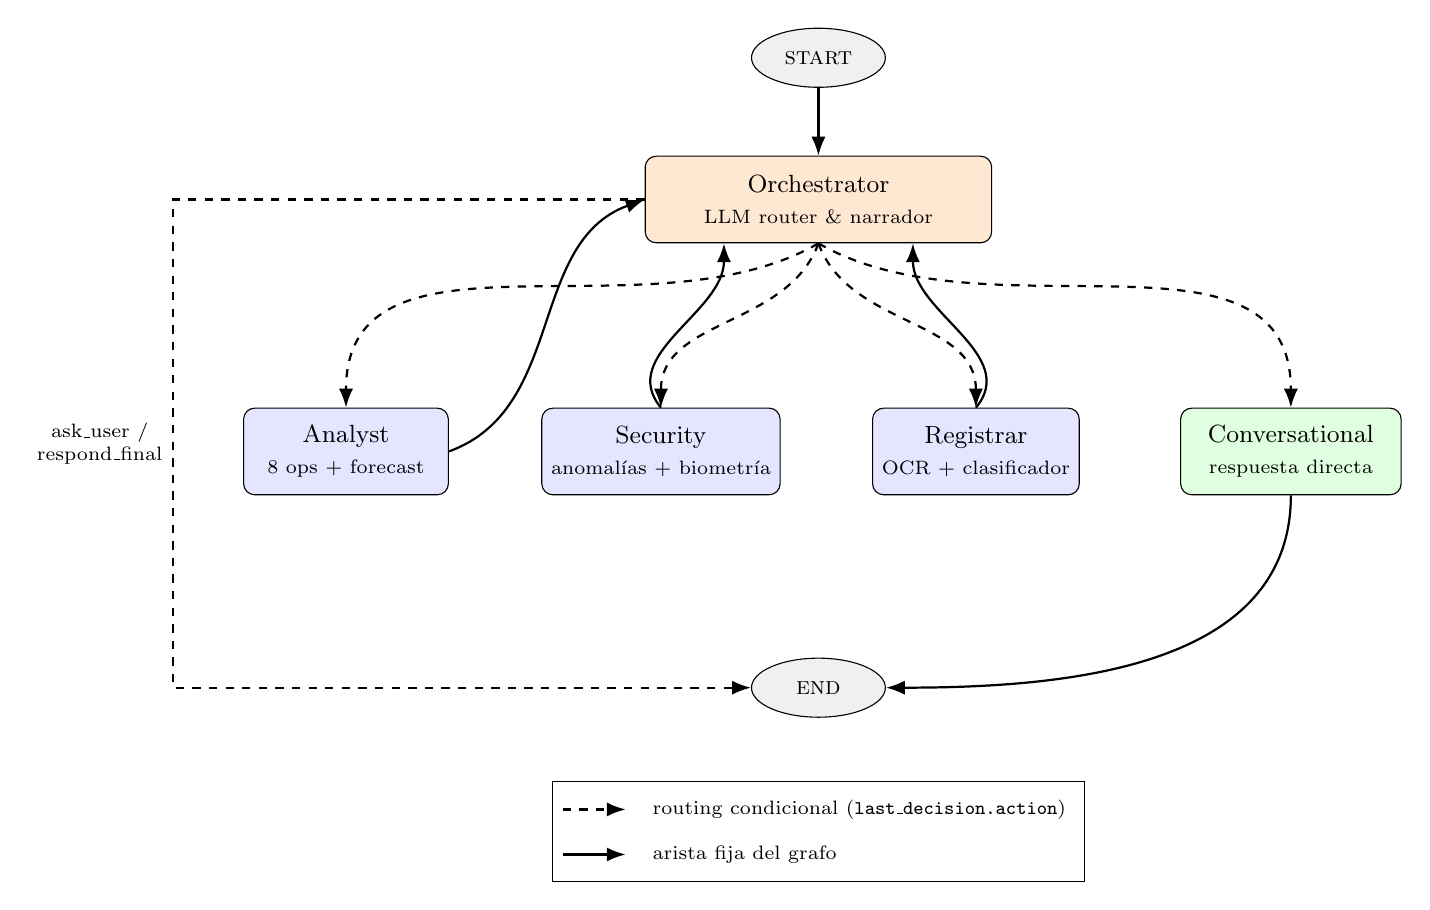
\begin{tikzpicture}[
    >={Latex[length=2.4mm]},
    every node/.style={font=\small},
    terminal/.style={ellipse, draw, fill=gray!12, minimum width=1.7cm, minimum height=0.75cm},
    orch/.style={rectangle, draw, rounded corners, fill=orange!18,
                 minimum width=4.4cm, minimum height=1.1cm, align=center},
    agent/.style={rectangle, draw, rounded corners, fill=blue!10,
                  minimum width=2.6cm, minimum height=1.1cm, align=center},
    convo/.style={rectangle, draw, rounded corners, fill=green!12,
                  minimum width=2.8cm, minimum height=1.1cm, align=center},
    route/.style={->, thick, dashed},
    back/.style={->, thick},
    final/.style={->, thick, dashed}
]

    % --- Fila 0: START ---
    \node[terminal] (start) at (0, 0) {\textsc{start}};

    % --- Fila 1: Orchestrator ---
    \node[orch] (orch) at (0, -1.8)
        {Orchestrator\\\scriptsize{LLM router \& narrador}};

    % --- Fila 2: Agentes (cuatro columnas, centradas en x=0) ---
    \node[agent] (analyst)   at (-6.0, -5.0) {Analyst\\\scriptsize{8 ops + forecast}};
    \node[agent] (security)  at (-2.0, -5.0) {Security\\\scriptsize{anomalías + biometría}};
    \node[agent] (registrar) at ( 2.0, -5.0) {Registrar\\\scriptsize{OCR + clasificador}};
    \node[convo] (conv)      at ( 6.0, -5.0) {Conversational\\\scriptsize{respuesta directa}};

    % --- Fila 3: END ---
    \node[terminal] (end) at (0, -8.0) {\textsc{end}};

    % --- Aristas ---
    % START -> Orchestrator
    \draw[back] (start) -- (orch);

    % Routing condicional (orchestrator -> especialistas)
    \draw[route] (orch.south) to[out=-150, in=90] (analyst.north);
    \draw[route] (orch.south) to[out=-110, in=90] (security.north);
    \draw[route] (orch.south) to[out=-70,  in=90] (registrar.north);
    \draw[route] (orch.south) to[out=-30,  in=90] (conv.north);

    % Retorno de especialistas al orquestador (arista fija)
    \draw[back] (analyst.east)    to[out=20,  in=200] (orch.west);
    \draw[back] (security.north)  to[out=130, in=-90] ($(orch.south)+(-1.2,0)$);
    \draw[back] (registrar.north) to[out=50,  in=-90] ($(orch.south)+(1.2,0)$);

    % Conversational -> END (arista fija)
    \draw[back] (conv.south) to[out=-90, in=0] (end.east);

    % Orchestrator -> END (ask_user / respond_final) — ruta exterior por la
    % izquierda, pasando fuera del nodo Analyst (x = -6.0, ancho 2.6).
    \coordinate (askL) at (-8.2, -1.8);
    \coordinate (askD) at (-8.2, -8.0);
    \draw[final] (orch.west) -- (askL) --
        node[left, font=\scriptsize, align=center]
        {ask\_user /\\respond\_final} (askD) -- (end.west);

    % --- Leyenda ---
    \matrix [draw, below=0.8cm of end, row sep=3pt, column sep=6pt,
             nodes={font=\scriptsize, anchor=west}] {
        \draw[route] (0,0) -- (0.8,0); & \node {routing condicional (\texttt{last\_decision.action})}; \\
        \draw[back]  (0,0) -- (0.8,0); & \node {arista fija del grafo}; \\
    };

\end{tikzpicture}
\end{document}
